\label{sec:cost}
\label{sec:opt-eval}
\bi{\emph{Maintenance and optimization.} After the population restatement, repairing each definition once uses \PpMavraMaintS\,s of database time versus \PpPrivateMaintS\,s for private copies. Non-breaking updates and repairs cost \AmMaintBenignS/\AmMaintRepairS\,s end to end; discarding knowledge on every write costs \ScenRelearnTok\,M relearning tokens. On one-million-row retail, \OptPublished{} of \OptDefs{} definitions receive equivalent key-range rewrites, saving \OptSaveMin--\OptSaveMax\% query time (mean \OptSaveMean\%); each paired mean-difference 95\% interval is below zero. Rewrites match \OptPeriods{} periods and are adopted by \OptHoldAdopted/\OptHoldTasks{} held-out queries. In a separate four-definition test, date re-keying invalidates every rewrite; fallback takes at most \PbFallbackMsMax\,ms and all \PbAnswers{} subsequent answers are correct (stale rewrites err by up to \PbStaleErrMax\%).}
{\emph{维护与优化。}群体更正后，每个定义修复一次使用 \PpMavraMaintS\,s 数据库时间，私有副本需 \PpPrivateMaintS\,s；正常更新／修复的端到端开销为 \AmMaintBenignS／\AmMaintRepairS\,s，每写即丢弃需 \ScenRelearnTok\,M token 重学。百万行零售中，\OptDefs{} 个定义中的 \OptPublished{} 个获得等价键区间改写，查询时间减少 \OptSaveMin--\OptSaveMax\%（均值 \OptSaveMean\%），各配对均值差的 95\% 区间均低于零。改写匹配 \OptPeriods{} 个期间，被 \OptHoldAdopted／\OptHoldTasks{} 条留出查询采用。独立四定义测试中，日期重新编键使全部改写失效；回退不超过 \PbFallbackMsMax\,ms，随后 \PbAnswers{} 个答案均正确，过期改写最高误差 \PbStaleErrMax\%。}
\begin{figure}[t]
\centering
\ifbilingual
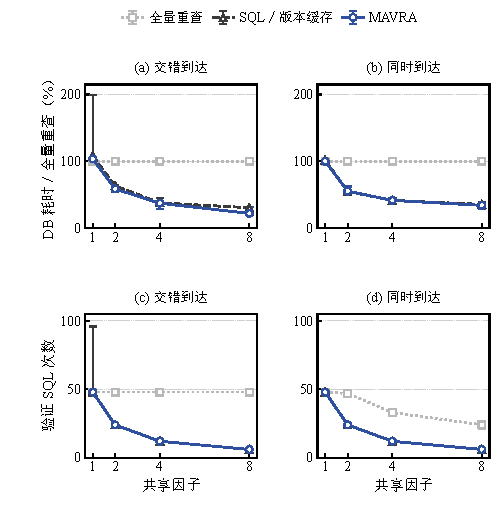
\includegraphics[width=\linewidth]{figures/fixed-sharing-zh}
\else
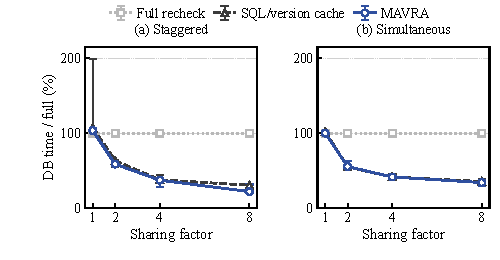
\includegraphics[width=\linewidth]{figures/fixed-sharing}
\fi
\caption{\bt{Validation time at fixed definition count, relative to matched full recheck. Points are three-block medians; error bars span all three observations.}{固定定义数下相对匹配全量重查的验证耗时。点为三轮中位数，误差棒覆盖全部三次观测。}}
\label{fig:fixed-sharing}
\Description{Two line charts compare full recheck, SQL/version cache, and MAVRA under staggered and simultaneous arrivals with a common vertical scale. Sharing factors are 1, 2, 4, and 8 definitions per table pair. The no-overlap SQL-cache outlier at about 199 percent of full-recheck database time is retained. Error bars are observed ranges, not confidence intervals. Validation query counts are reported in the text.}
\end{figure}

\bi{\emph{Shared validation.} Figure~\ref{fig:fixed-sharing} fixes 16 definitions over 16/8/4/2 active table pairs (sharing factors 1/2/4/8), eight agents and 128 requests per cell, and 100k rows per fact table. All 16 pairs receive identical warmup, benign writes and version invalidations. Three randomized blocks yield 72 cells and \MeBRequests{} valid requests. Staggered \system{} checks fall from 48 to six while full recheck stays at 48. At factor eight, matched database times are \MeBStagMavra\%/\MeBBurstMavra\% for \system{} and \MeBStagCache\%/\MeBBurstCache\% for SQL caching (staggered/simultaneous). Both reuse exact checks; full recheck also coalesces simultaneous requests. One factor-one cache run refreshes twice (96 checks; 199.36\%). Times include metadata; active tables decrease with sharing.}
{\emph{共享验证。}图~\ref{fig:fixed-sharing}固定 16 个定义，映射到 16／8／4／2 个活跃表对（共享因子 1／2／4／8），每格八智能体、128 请求，每事实表 100k 行。全部 16 表对接受相同预热、良性写入和版本失效。三轮随机顺序产生 72 格、\MeBRequests{} 次有效请求。交错到达时 \system{} 检查从 48 降至六次，整定义重查保持 48 次。因子八时，相对匹配重查的数据库耗时为 \system{} 的 \MeBStagMavra\%／\MeBBurstMavra\%、SQL 缓存的 \MeBStagCache\%／\MeBBurstCache\%（交错／同时到达）。两者复用相同检查，整定义重查也合并同时到达请求；因子一的一次缓存运行刷新两次（96 检查、199.36\% 耗时）。数据库耗时含元数据；活跃表集合随共享缩小。}

